\chapter{Hardware Description}
To accurately implement the  load emulation in real-time a multiple processor
system may required. Fig.~\ref{overall} shows the block diagram of closely coupled DSP system. In this system separate processors are employed to carry out data acquisition, communication and control for load emulation. This system is based on Texas TMS320vc33 DSP. In order to get flexible I/O interface and data acquisition, this system has two processors and a FPGA on single board. It provides interface between the USB controller and the DSP via Link Interface Manager (LIM) using Texas MSP430F168 Micro controller. Communication between PC's USB port and MSP 430F168 micro controller is done using Texas USB controller TUSB3210. DSP is used as a controller which executes the algorithms that control the converter via ASIC. Micro controller carries out data acquisition, storing real-time data, also  can  be used to transfer the data to PC for graphical display. The LIM is also interfaced to sensor unit for data acquisition.
ASIC is used to carry out the pulse width modulation (PWM) for controlling  the converter.\par
\begin{figure}[ht]
\centering
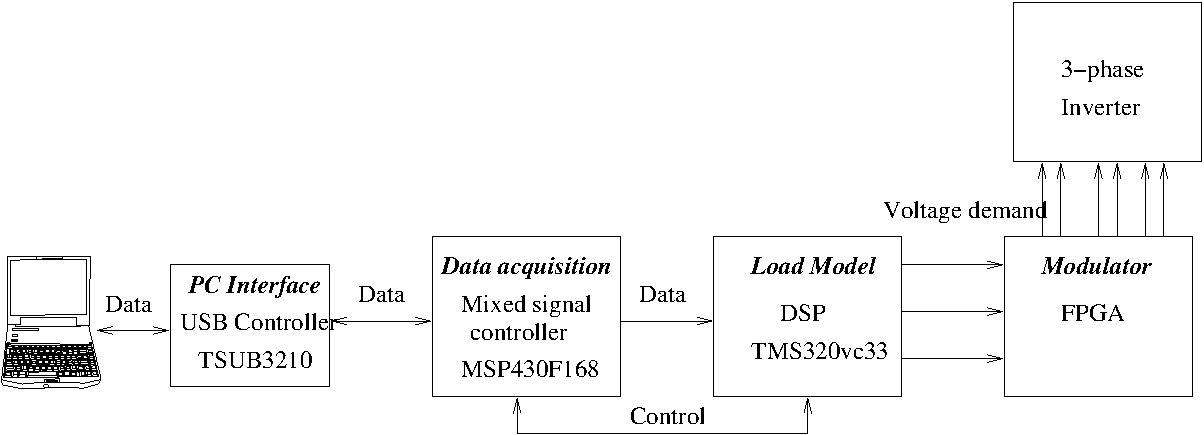
\includegraphics[width=6in]{overall.pdf}
\caption{Block diagram of closely coupled DSP system.}
\label{overall}
\end{figure}
\emph {The system requires the following I/O functions:}\\
(a) Sampling of three line currents: Even if two line currents are sufficient due to the symmetrical nature of the load, it is important to have the third line current also sampled for the evaluation purposes. This requires three A/D converter inputs.\\
(b) Sampling of three line voltages: Even if two line voltages are sufficient due to the symmetrical nature of the load, it is important to have the third line voltages also sampled for the evaluation purposes. This requires three A/D converter inputs.\\
(c) DC link voltage sampling: Since DC link voltage is used as a measured signal in the control algorithms, this will require another A/D converter input.
